%\documentclass[draft]{article}

\documentclass[pdftex,12pt,letterpaper]{article}
\usepackage[margin=1in]{geometry}
\usepackage[pdftex]{graphicx}
\usepackage{amsmath}
\usepackage[font=footnotesize,labelfont=bf,margin=0.5in,justification=justified, singlelinecheck=on]{caption}
\usepackage{float}

% Allow superscript citations
\usepackage[superscript]{cite}

% Captions
%\usepackage[margin=0.5in,justification=justified, singlelinecheck=on]{caption}
\captionsetup[table]{singlelinecheck=on}

\newcommand{\HRule}{\rule{\linewidth}{0.5mm}}

\begin{document}

% % % % % % % % % % % % % % % % % % % % % % % % % % % % % % % % % % % % % % % %
% % % % % % % % % % % % % % % % % % % % % % % % % % % % % % % % % % % % % % % %
		% 						         Laboration														          %
% % % % % % % % % % % % % % % % % % % % % % % % % % % % % % % % % % % % % % % %
%% % % % % % % % % % % % % % % % % % % % % % % % % % % % % % % % % % % % % % % %

\begin{titlepage}
\begin{center}

% Upper part of the page. The '~' is needed because \\
% only works if a paragraph has started.

\includegraphics[width=0.5\textwidth]{./logo}~\\[1cm]

\vspace{4cm}

\textsc{\Large Biomedical Instrumentation}\\[0.5cm]

% Title
\HRule \\[0.4cm]
{ \huge \bfseries ECG Amplifier Laboration \\[0.4cm] }

\HRule \\[1.5cm]

% Author and supervisor
\noindent
\begin{minipage}{0.4\textwidth}
\begin{flushleft} \large
\emph{Authors:}\\
Courtney \textsc{Keeler} \\
Arsalan \textsc{Latif}
\end{flushleft}
\end{minipage}%
\begin{minipage}{0.4\textwidth}
\begin{flushright} \large
\emph{Professor:} \\
Dr.~Sabine \textsc{Reinfeldt} \\
\emph{Teaching Assistant:} \\
Cristina \textsc{Rigato}
\end{flushright}
\end{minipage}

\vfill

% Bottom of the page
{\large \today}

\end{center}
\end{titlepage}

\section{Introduction}

Electrocardiography (ECG) amplifiers are common  medical devices that are used to measure the electrical activity of a patient's heart. The body surface potentials that are physically measured by the device are very small in amplitude, and therefore require an amplifier that attenuates noise while amplifying the desired signal, all while protecting both the patient and the instrument. In this lab, an ECG amplifier circuit was analyzed, built, and verified on a patient in the lab.

\section{Design and Simulation}

The basic requirements for ECG circuitry are high input impedance, high gain for the desired frequency range, and high common mode rejection ratio (CMRR). These parameters are set by the circuit designer through choice of component values. The final component values are summarized in Table \ref{table:values}. Component labels correspond to those shown in Figure \ref{fig:circuit},  the overall schematic of the ECG amplifier circuit.


\begin{table}[H]
\begin{center}
    \begin{tabular}{ | l | l | }
    \hline
    Label & Value \\ \hline
    $R_{in}$ & 100 k$\Omega$ \\ \hline
    $R_1$ & 1.2 k$\Omega$ \\ \hline
    $R_2$ & 22 k$\Omega$  \\ \hline
    $R_3$ & 1 k$\Omega$  \\ \hline
    $R_4$ & 22 k$\Omega$ \\ \hline
    $R_5$ & 3.3 M$\Omega$  \\ \hline
    $R_6$ & 10 k$\Omega$  \\ \hline
    $R_7$ & 10 k$\Omega$ \\ \hline
    $R_8$ & 10 k$\Omega$  \\ \hline
    $R_9$ & 10 k$\Omega$  \\ \hline
    $C_1$ & 1 $\mu$F \\ \hline
    $C_2$ & 150 nF  \\ \hline
    $C_3$ & 68 nF  \\
    \hline
    \end{tabular}
    \caption{Final component values for the ECG amplifier circuit.}
    \label{table:values}
\end{center}
\end{table}


\begin{figure}[H]
\begin{center}
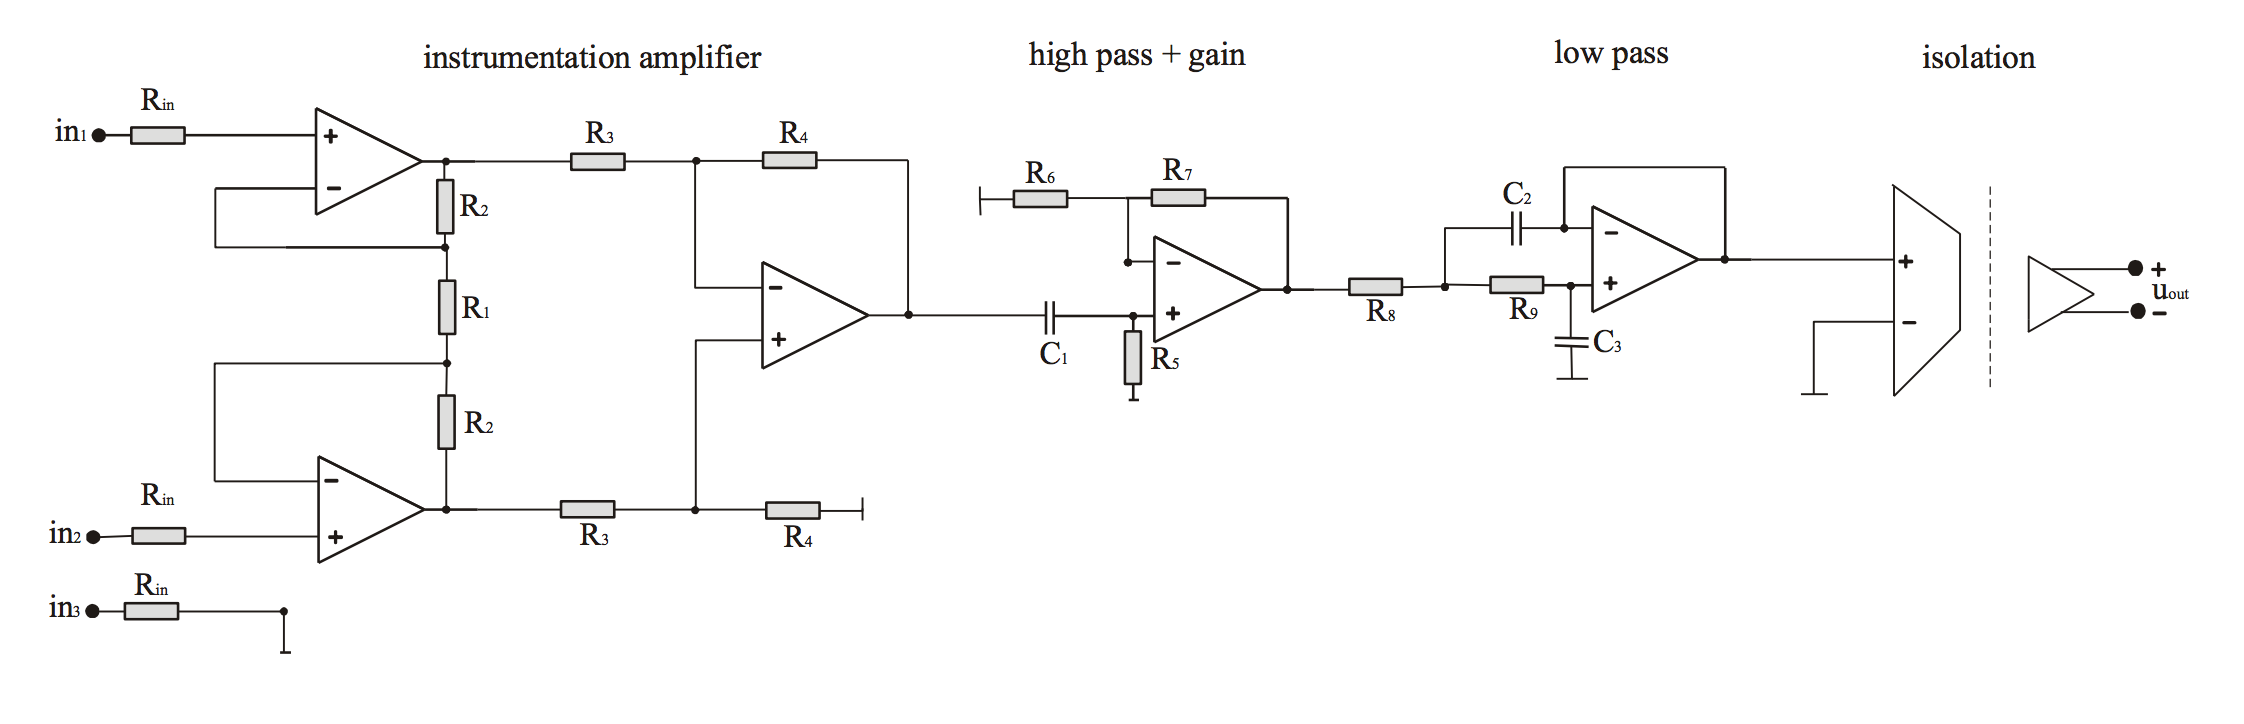
\includegraphics[scale=.35]{ECG_circuit.png}
\caption{Schematic of the circuitry used to amplify ECG signals in the laboratory. In the constructed circuit, there is a unity gain non-inverting voltage follower between the instrumentation amplifier and the first filter. This is because the op amp ICs come in pairs of two, so the circuit must have an even number of op amps (not including the isolation amplifier).}
\label{fig:circuit}
\end{center}
\end{figure}

In total, the gain of the ECG amplifier should be 1750. However, it is bad practice to apply all of the gain at a single amplification stage, so for this reason the gain is spread between the entire instrumentation amplifier and high pass filter. The first stage of the circuit, the instrumentation amplifier, was designed to have the following gain:
$$
G_1 = \frac{2R_2+R_1}{R_1}(\frac{R_4}{R_3})
$$
$$
G_1 = \frac{2(22k)+1.2k}{1.2k}(\frac{22k}{1k}) = 828.67.
$$
The gain of the second stage of the circuit, the high pass filter,  was designed by the following equation:
$$
G_2 = 1 + \frac{R_7}{R_6}
$$
$$
G_2 = 1 + \frac{10k}{10k} = 2.
$$
This gives a total gain of
$$
G_{total} = (G_1)(G_2) = (828.67)(2) = 1657.34.
$$

The final stage of the circuit, the Sallen-Key low pass filter, was designed for unity gain. However, special consideration had to be given to the component values in order to create Butterworth behavior. This means that the magnitude of the frequency response for the pass band is flat. A second order Butterworth filter in particular has a maximally flat passband. For the Sallen-Key filter in the ECG circuit, the following change of variables is made:
$$
R_8 = mR
$$
$$
R_9 = R
$$
$$
C_2 = mC
$$
$$
C_3 = C.
$$
The following variables are also defined:
$$
Q = \frac{\sqrt{mn}}{m+1}
$$
$$
\omega_0 = 2\pi f_0 = \frac{1}{RC\sqrt{mn}}.
$$
For a second order Butterworth, $Q = 1/\sqrt{2}$. It is also desired for the ECG application that $f_0 = 200$ Hz. Even with this information, there are too many variables to solve for both capacitor and both resistor values. Therefore, it is arbitrarily chosen that $m=1$, which implies $R_8 = R_9$. The choice of resistance value is again arbitrary, and here set as 10 k$\Omega$. Now the capacitance values can be solved for:
$$
\frac{1}{\sqrt{2}} = \frac{\sqrt{n}}{2} \rightarrow n = 2
$$
$$
2\pi 200 = \frac{1}{(10k)C(\frac{2}{\sqrt{2}})} \rightarrow C = C_3 = .0563 \mu F
$$
$$
C_2 = nC = .1126 \mu F.
$$
In practice, these values for the high pass capacitors were rounded to the closes standard values. The values that were used in the constructed circuit can be seen in Table \ref{table:values}.

In theory, the values of $R_{in}$ should be chosen such that the input impedance of the ECG amplifier circuit is sufficiently high. However, in practice if these values are too large, there is no signal seen at the output of the $R_{in}$ resistors. This is the reason for the value of 100 k$\Omega$ seen in Table \ref{table:values}.

\subsection{AC Analysis}

The final ECG circuit was simulated in two configurations in order to observe the direct mode (DM) and common mode (CM) signals. These two wiring schemes are illustrated in Figure \ref{fig:DM_CM}.

\begin{figure}[H]
\begin{center}
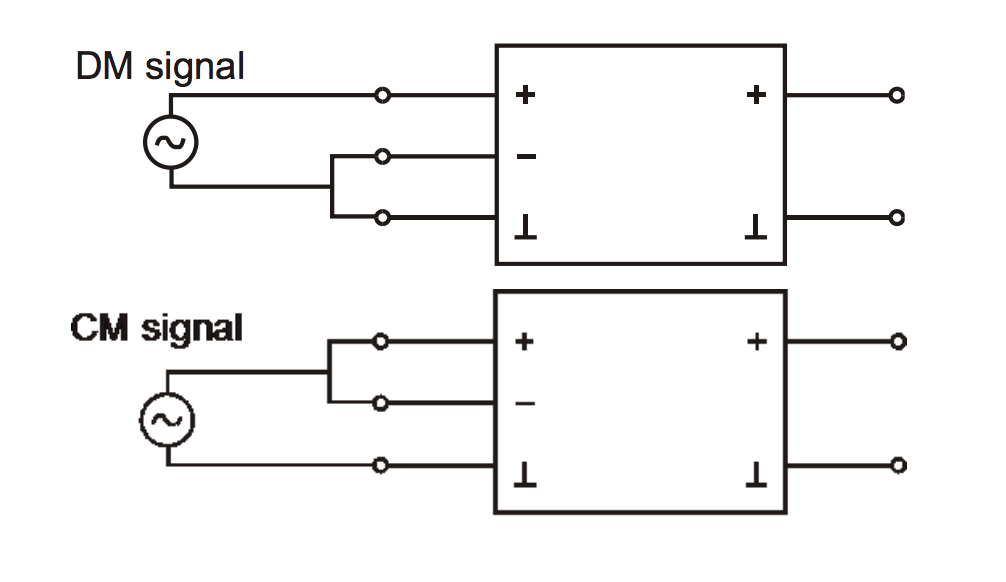
\includegraphics[scale=.5]{DM_CM.png}
\caption{Schematic of the input configurations for measuring DM and CM signals.}
\label{fig:DM_CM}
\end{center}
\end{figure}

First, the DM signals were investigated. It is desired to have a large DM signal gain; the previous section demonstrated that the gain of the ECG amplifier circuit should be just over 1600. Figure \ref{fig:DM} shows the response of the circuit for a range of relevant frequencies. 

\begin{figure}[H]
\begin{center}
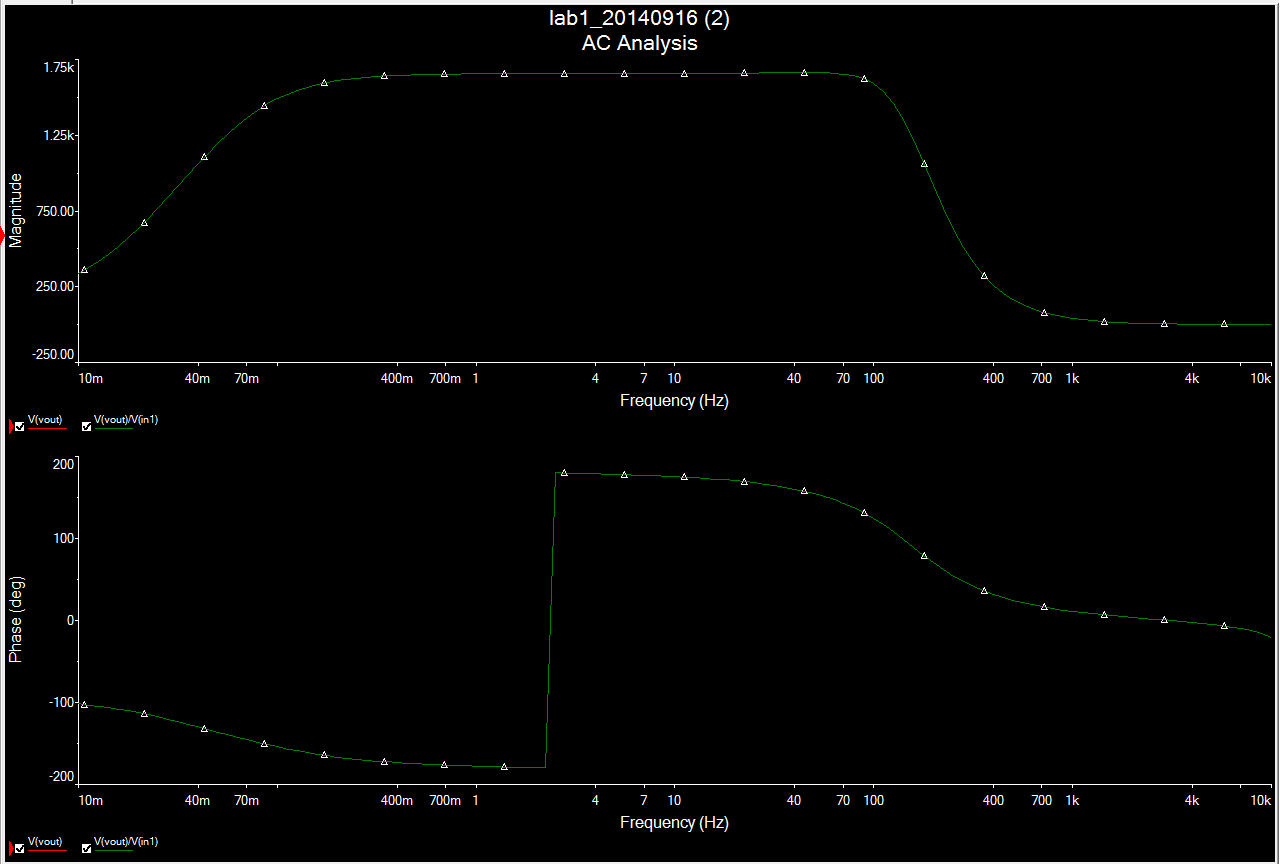
\includegraphics[scale=.35]{DM_analysis.png}
\caption{AC analysis of the simulated ECG amplifier circuit in DM measurement configuration. Notice the flat top of the magnitude spectrum. This is due to the use of a second order Butterworth filter.}
\label{fig:DM}
\end{center}
\end{figure}

It can be seen that within the range of about .4 - 100 Hz the DM signal is amplified by approximately 1750. This fits the original design requirement that the ECG amplifier have a DM gain of over 1000.

Figure \ref{fig:CM} shows the response of the circuit to CM signals over a range of simulated frequencies.
\begin{figure}[H]
\begin{center}
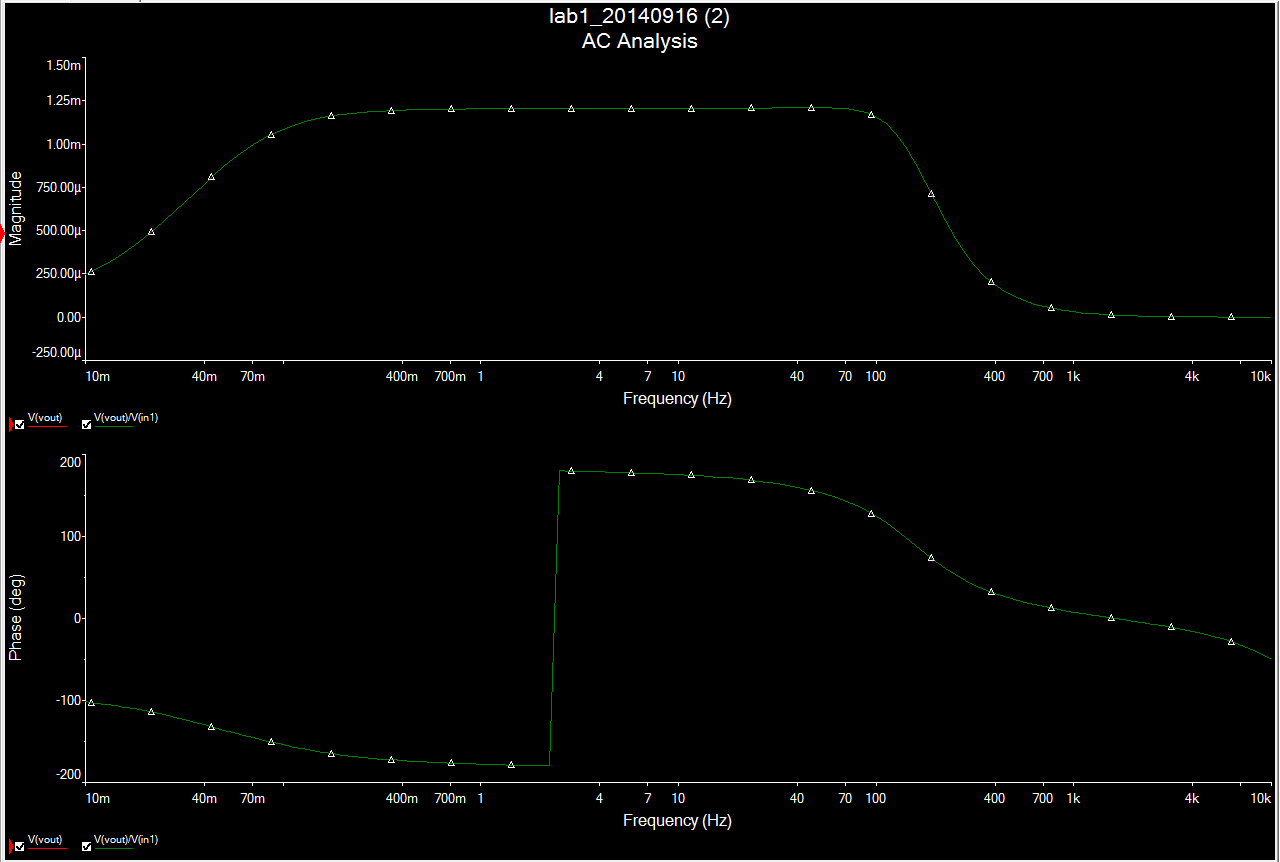
\includegraphics[scale=.35]{CM_analysis.png}
\caption{AC analysis of the simulated ECG amplifier circuit in CM measurement configuration.}
\label{fig:CM}
\end{center}
\end{figure}
In this case, a very small gain is desired. The maximum gain of these signals from the designed circuit occurs in the frequency range of about .4 - 100 Hz, and the magnitude of the gain is approximately 0.00125. In order to calculate if this value is sufficiently small, one must compute the common mode rejection ratio (CMRR). This is the ratio of the DM gain to the CM gain, as seen below:
$$
CMRR = \frac{A_{DM}}{A_{CM}} = \frac{1656.4}{.0012045} = 1375176.42
$$
This value is sufficiently large, which means that the DM and CM gains of the designed circuit are appropriate.

Figure \ref{fig:3DB} shows the frequency response of the DM circuit again, this time with the magnitude plotted in dB. This is so that the $\pm$3 dB cutoff points are easier to identify. These corner frequencies are important to know because they correspond to the range over which the above CMRR is valid. Ideally, the upper and lower corner frequencies encompass the range of frequencies present in an ECG signal so that nothing of importance is attenuated during measurement.
\begin{figure}[H]
\begin{center}
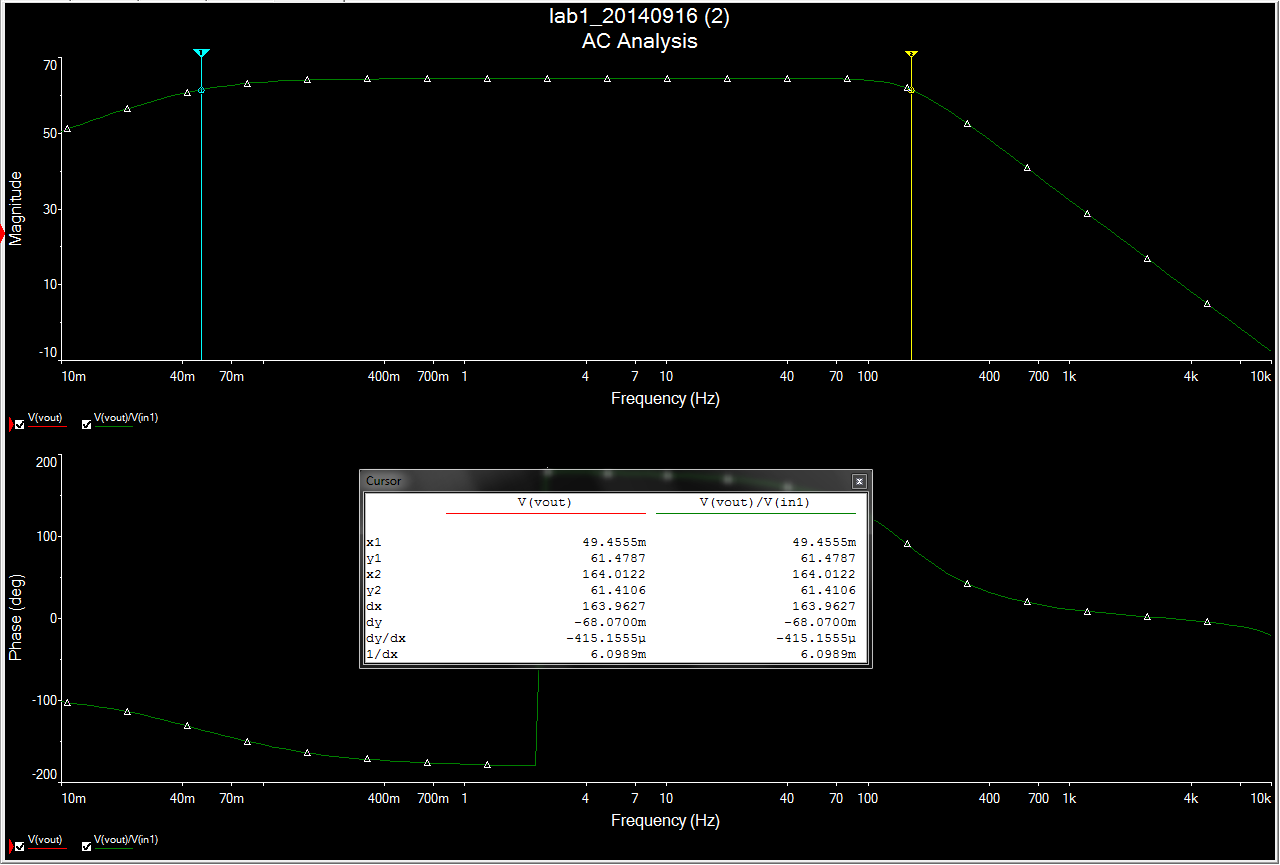
\includegraphics[scale=.35]{3db_analysis.png}
\caption{AC analysis of the simulated ECG amplifier circuit in DM measurement configuration. The y-axis is plotted in decibels in order to easily find the $\pm$3dB cutoff frequencies. Cursors 1  and 2 are placed at the lower and upper corner frequencies, respectively.}
\label{fig:3DB}
\end{center}
\end{figure}
According to Figure \ref{fig:3DB}, the lower corner frequency occurs at .049 Hz and the upper corner frequency is at 164 Hz, which is sufficient to capture the majority of the frequency components of an ECG signal.

\section{Construction and Data Acquisition}

After approving a schematic of the component placement, the ECG amplifier was soldered onto a permanent Vero board. The circuit was built with a TL072 (operational amplifier), ISO124 (isolation amplifier), resistances, capacitances, 9V batteries and connectors. The NI Elvis platform is used as an oscilloscope and digital multi meter. It was also used to check the proper functioning of each component i.e. the operational amplifiers, filters and isolation amplifier by generating a known signal (10 mV, 30Hz) and observing the output across each component. 

Before the amplifier could be used to measure cardiac bio-potentials; the DC offset, gain, DM signal and CM signal needed to be measured. The DM and CM signal gains were measured for a range of frequencies using the NI Elvis platform to both generate a known signal and measure the resulting signal at the output of the Butterworth filter (the isolation amplifier was only connected to the circuit when it was used to measure the ECG signal of a patient). The DC offset was also measured using the same NI Elvis platform with the circuit in the DM measurement configuration. 
   
Once the correct functionality of each functional block and relevant parameters were verified, it was decided to move towards acquisition of ECG bio-potentials. The amplifier has three input electrodes that were connected to the volunteer as shown in Figure \ref{fig:setup}. The positive electrode was placed near the dipole of the heart while the negative electrode was placed further away but at same vertical height as the positive electrode. The third electrode served as ground and was placed on the hip. The outputs of the isolation amplifier were connected to a digital to analog converter (DAC) and the ECG waveform was consequently visualized on the computer through a LABVIEW program.

\begin{figure}[H]
\begin{center}
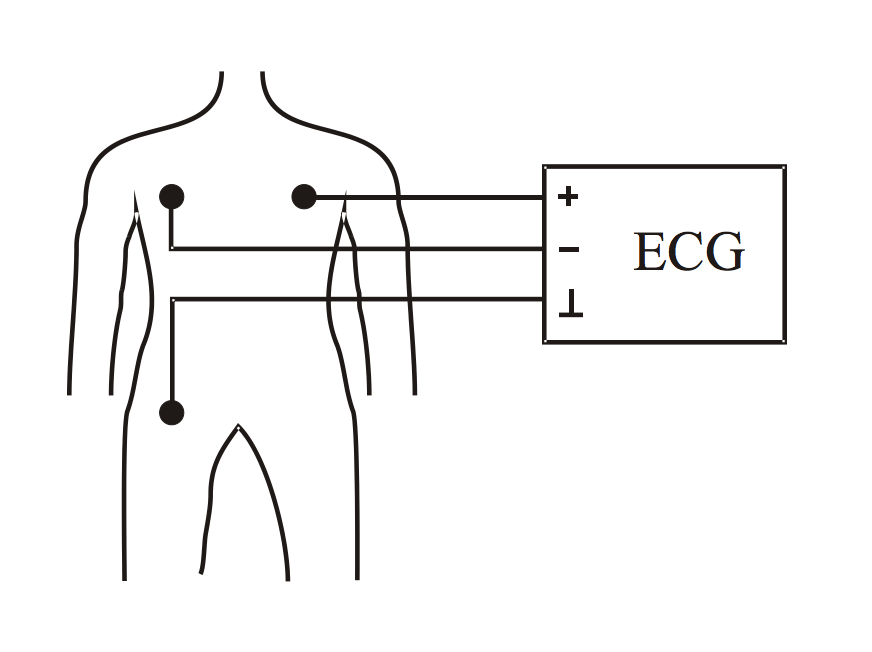
\includegraphics[scale=.5]{setup.png}
\caption{Schematic of the electrode placement for the acquisition of ECG signals in the laboratory.}
\label{fig:setup}
\end{center}
\end{figure}

\section{Results}

The measured gains for the DM and CM configuration over a range of relevant frequencies should in theory match the magnitude plots seen in Figures \ref{fig:DM} and \ref{fig:CM}. In reality, there are sources of noise and tolerances on components that cause deviations in the actual values from those expected. Figure \ref{fig:DM_response} shows the amplification of DM signals over the relevant frequency range.
\begin{figure}[H]
\begin{center}
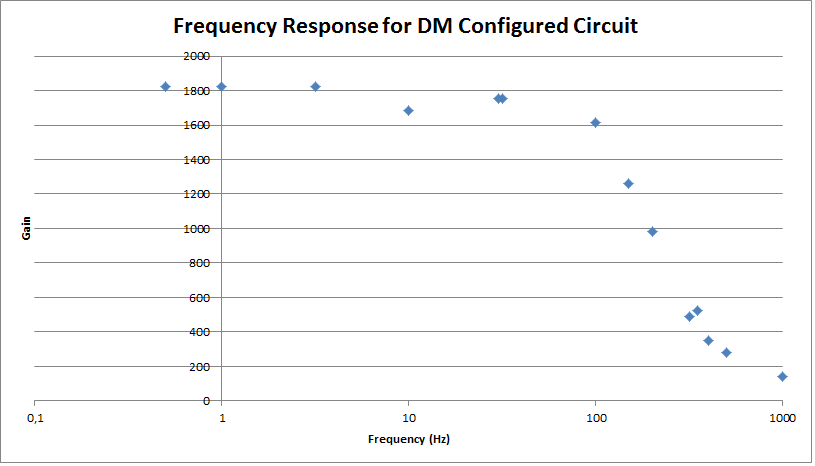
\includegraphics[scale=.5]{fig1.png}
\caption{Frequency response of the constructed ECG amplifier in DM mode.}
\label{fig:DM_response}
\end{center}
\end{figure}
Notice that the passband region is not flat, as was desired by designing the low pass filter as a second order Butterworth. This is an example of the difference between a simulated and physically realized circuit. However, the overall shape still matches the expected value, and the maximum amplification of 1822 matches the expected value of 1657 relatively well. 

Further, the frequency response of the CM configuration, as seen in Figure \ref{fig:CM_response}, matches the expected values for the small range that could be measured in lab.
\begin{figure}[H]
\begin{center}
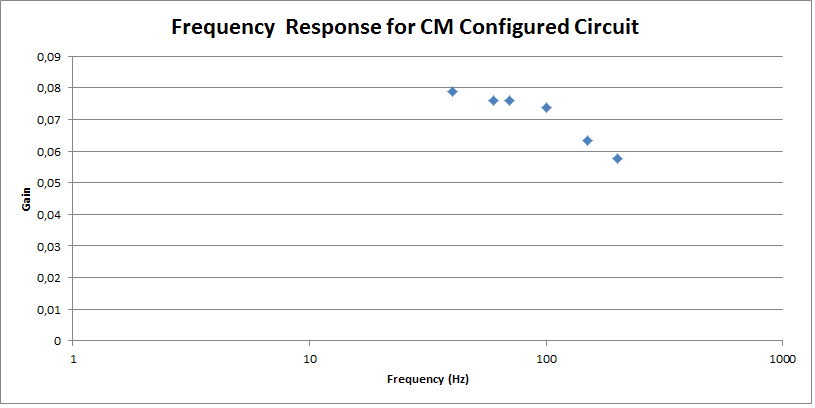
\includegraphics[scale=.5]{fig2.png}
\caption{Frequency response of the constructed ECG amplifier in CM mode.}
\label{fig:CM_response}
\end{center}
\end{figure}
In practice, it was very difficult to produce a large enough amplitude signal that generate an output signal discernible from 50 Hz power line distortion while the ECG circuit was in the CM configuration. For this reason, only a small range of frequency values could be measured for the actual frequency response. It can be seen that the actual maximum CM amplification value, 0.08, is higher than the simulated value, .00125. This is because the simulation is a best case scenario for the performance of the circuit.

With real values of DM and CM gain from the constructed circuit, it is possible to calculate the real CMRR, as below:
$$
CMRR = \frac{A_{DM}}{A_{CM}} = \frac{1822}{.08} = 22775.
$$
Here it can be seen that what seems like a 'fairly close' agreement in CM amplification values can lead to a very large decrease in the quality of the CMRR. However, the constructed circuit will still function to acquire ECG signals, albeit with a lower signal to noise ratio.

The DC offset was found to be 0 when the input offset was 0. However, when the input offset was changed to a positive value an rise in output offset was noticed. However, this offset settled back down to 0 within several seconds. This behavior can be reasoned with the presence of capacitors in the circuit. 

A three lead ECG consist of five points; P wave, QRS complex, T. In the captured ECG waveform, the P wave and the QRS complex are clearly distinguished, as highlighted in Figure \ref{fig:ECG}. To smooth the signal a notch filter of 50 Hz was applied through LABVIEW. 
\begin{figure}[H]
\begin{center}
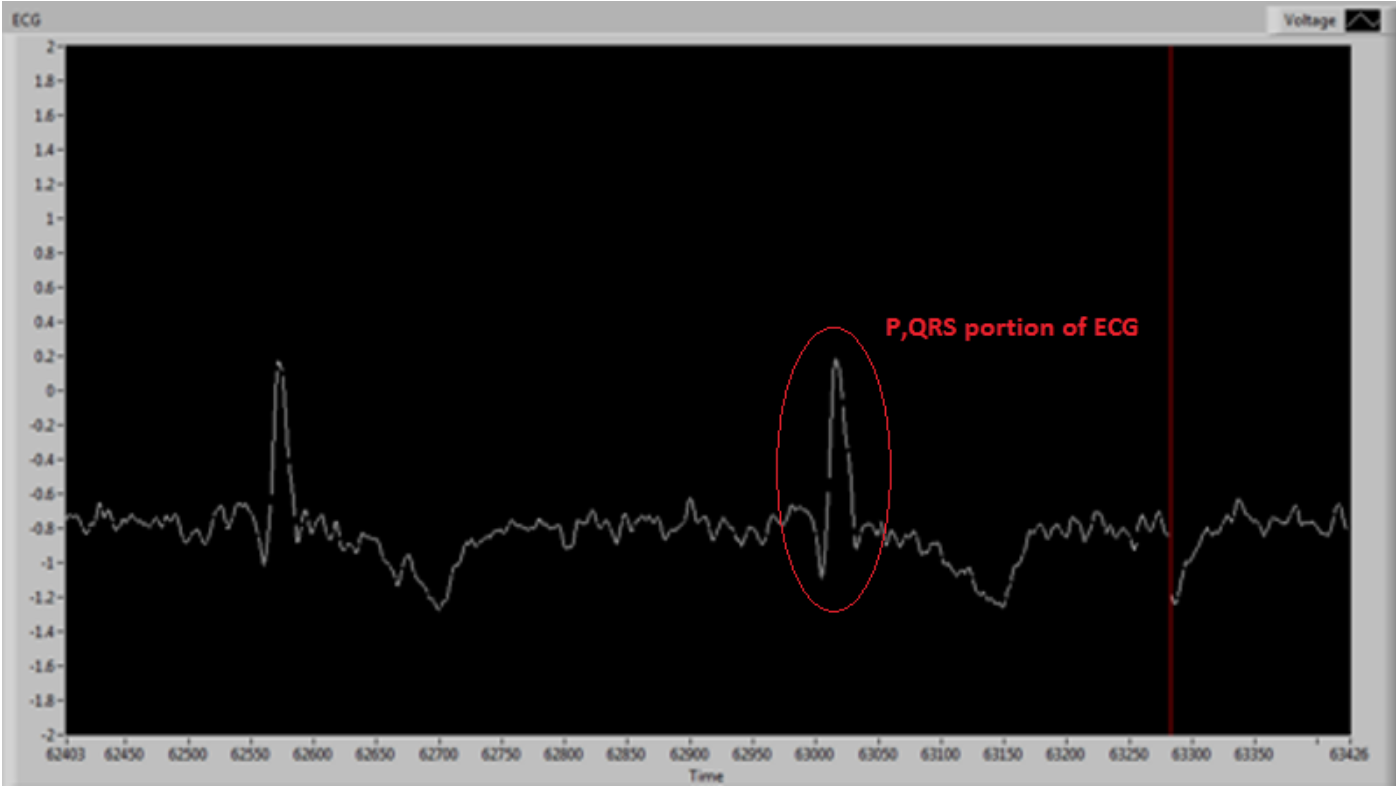
\includegraphics[scale=.6]{pqrst.png}
\caption{Captured and filtered waveform from the ECG amplifier circuit when hooked up to electrodes placed on a patient.}
\label{fig:ECG}
\end{center}
\end{figure}
The ST segment and the T wave of the ECG waveform are also present but are distorted due noise. This distortion in the signal comes from a variety of sources which include power line distortion and motion artifacts.

\section{Device Limitations}

The foremost limitation of the built amplifier is its inability to clearly differentiate the ST segment and the T wave. In the current circuit, the only biometric that can be determined is the beats per minute (BPM), found by examining the separation in time of subsequent QRS peaks. For some simple applications this is the only result of interest, and the circuit presented in this lab would be adequate. However, if more information is needed on the complete P,QRS,T waves, then the noise and power distortion will need to be better handled. This could be done through means such as shielding the device and electrodes. Another source of noise is motion artifact, which the current amplifier design is susceptible to. Motion artifact could be minimized by designing a device with shorter leads, or by asking the patient to lie down in a relaxed position while the measurements are being taken.

Three electrodes is also the minimum number of electrodes needed to detect cardiac bio-potentials. In order to acquire a more complete picture of the electrical activity of different regions of the heart, the number of electrodes detecting the cardiac bio-potentials must be increased.

\end{document}